\part*{Ejercicio 4}
Se nos solicitó medir los tiempos de propagación, rise time y fall time de una compuerta 74HC02 en vacío, y luego repetir el experimento implementando el circuito mostrado en la Figura \ref{4_fig3}. La compuerta NOR es una 74HC02 y las NAND son 74HC00.
%\begin{figure}[H]
%\centering
%\begin{circuitikz}[scale=1] \draw
(-1.4,0) to[short,*-o] (-2,0)
(0,0) node[nor port](myand1) {}
(myand1.in 1) -| (myand1.in 2)
(myand1.out) to[short] (0.5,0)
(2.5,3) node[nand port](nandgate1){}
(nandgate1.in 1) -| (nandgate1.in 2)
(2.5,1.5) node[nand port](nandgate2){}
(nandgate2.in 1) -| (nandgate2.in 2)
(2.5,0) node[nand port](nandgate3){}
(nandgate3.in 1) -| (nandgate3.in 2)
(2.5,-1.5) node[nand port](nandgate4){}
(nandgate4.in 1) -| (nandgate4.in 2)
(0.5,3) to[short,-] (0.5,-3)
(0.5,3)to[short,-*] (1.11,3)
(0.5,1.5) to[short,*-*] (1.11,1.5)
(0.5,0) to[short,*-*] (1.11,0)
(0.5,-1.5) to[short,*-*] (1.11,-1.5)
(nandgate1.out) -- (3,3)
to[R=1k] (4.5,3) to[empty led] (6.5,3)
(nandgate2.out) -- (3,1.5)
to[R=1k] (4.5,1.5) to[empty led,-*] (6.5,1.5)
(nandgate3.out) -- (3,0)
to[R=1k] (4.5,0) to[empty led,-*] (6.5,0)
(nandgate4.out) -- (3,-1.5)
to[R=1k] (4.5,-1.5) to[empty led,-*] (6.5,-1.5)
(0.5,-3) to[short] (3,-3)
to[R=560] (4.5,-3) to[empty led,-*] (6.5,-3)
(6.5,3) to[short] (6.5,-3.5)
(6.5,-3.5) node[ground]{}
;
\end{circuitikz}
%\caption{Circuito a implementar}
%\label{4_fig3} 
%\end{figure}

\begin{wrapfigure}{l}{6.5cm}
\begin{center}
\resizebox{.5\linewidth}{!}{\parbox{\linewidth}{\begin{circuitikz}[scale=1] \draw
(-1.4,0) to[short,*-o] (-2,0)
(0,0) node[nor port](myand1) {}
(myand1.in 1) -| (myand1.in 2)
(myand1.out) to[short] (0.5,0)
(2.5,3) node[nand port](nandgate1){}
(nandgate1.in 1) -| (nandgate1.in 2)
(2.5,1.5) node[nand port](nandgate2){}
(nandgate2.in 1) -| (nandgate2.in 2)
(2.5,0) node[nand port](nandgate3){}
(nandgate3.in 1) -| (nandgate3.in 2)
(2.5,-1.5) node[nand port](nandgate4){}
(nandgate4.in 1) -| (nandgate4.in 2)
(0.5,3) to[short,-] (0.5,-3)
(0.5,3)to[short,-*] (1.11,3)
(0.5,1.5) to[short,*-*] (1.11,1.5)
(0.5,0) to[short,*-*] (1.11,0)
(0.5,-1.5) to[short,*-*] (1.11,-1.5)
(nandgate1.out) -- (3,3)
to[R=1k] (4.5,3) to[empty led] (6.5,3)
(nandgate2.out) -- (3,1.5)
to[R=1k] (4.5,1.5) to[empty led,-*] (6.5,1.5)
(nandgate3.out) -- (3,0)
to[R=1k] (4.5,0) to[empty led,-*] (6.5,0)
(nandgate4.out) -- (3,-1.5)
to[R=1k] (4.5,-1.5) to[empty led,-*] (6.5,-1.5)
(0.5,-3) to[short] (3,-3)
to[R=560] (4.5,-3) to[empty led,-*] (6.5,-3)
(6.5,3) to[short] (6.5,-3.5)
(6.5,-3.5) node[ground]{}
;
\end{circuitikz}}}
\caption{Circuito a implementar}
\label{4_fig3}
\end{center}
\end{wrapfigure}

A continuación se nos solicitó aumentar la frecuencia del generador de señales a 100kHz y medir la tensión de alimentación, y repetir la experiencia conectando capacitores de desacople en los terminales de alimentación de los integrados.
Los resultados obtenidos para los tiempos de propagación, rise time y fall time de la compuerta 74HC02 en vacío fueron:

\begin{figure}[H]
\begin{flushright}
\begin{tabular}{|c|c|}
\hline 
Tiempo de propagación & 9.39 nseg \\ 
\hline 
Rise time & 9.93 nseg \\ 
\hline 
Fall time & 35.5 nseg \\ 
\hline 
\end{tabular}
\end{flushright}
\end{figure}

Cuando se implementó el circuito mostrado en la Figura \ref{4_fig3}, los valores obtenidos fueron:

\begin{center}
\begin{tabular}{|c|c|}
\hline 
Tiempo de propagación & 12.7 nseg \\ 
\hline 
Rise time & 38.8 nseg \\ 
\hline 
Fall time & 32.9 nseg \\ 
\hline 
\end{tabular}
\end{center}

Se observa que el tiempo de propagación y el fall time se ven ligeramente afectados. No así el rise time, el cuál es aproximadamente 4 veces mayor cuando se carga la salida de la compuerta NOR con el circuito mostrado.

\bigskip
Seguidamente se aumentó la frecuencia del generador de señales a 100kHz y se midió la señal de alimentación. La Figura \ref{4_fig1} muestra unos pequeños sobrepicos que coinciden con los flancos de la señal de entrada. Estos sobrepicos se poducen porque cuando las compuertas conmutan producen una demanda de corriente significativa, la cual es provista por la fuente de alimentación. La linea de alimentación de los integrados posee una impedancia despreciable cuando no hay variaciones de corriente en el circuito, sin embargo cuando conmutan las compuertas y las fluctuaciones en la corriente son repentinas, los efectos de la impedancia se manifiestan, y aparecen sobrepicos de tension en la linea.
<<<<<<< HEAD
\begin{figure}[H]
\centering
\includegraphics[scale=0.2]{ejercicio4/imagenes/sin_capacitor.png}
\caption{Tensión en el terminal de alimentacion del 74HC02 sin capacitor}
\label{4_fig1} 
\end{figure}
=======
%\begin{figure}[H]
%\centering
%\includegraphics[scale=0.2]{imagenes/sin_capacitor.png}
%\caption{Tensión en el terminal de alimentacion del 74HC02 sin capacitor}
%\label{4_fig1} 
%\end{figure}
>>>>>>> 28770c77f59a955116c90b016e0ebd8b5d5b6c49

Para suavizar este efecto, se colocaron, como indica la consigna, capacitores de desacople en los terminales de alimentación de los circuitos integrados. Como muestra la Figura \ref{4_fig2}, el efecto es contrarrestado de forma significativa. De esta forma, cuando el circuito demanda un flujo de corriente repentinamente, el capacitor provee la corriente al integrado y no se producen cambios repentinos de corriente en la linea de alimentación.

%\begin{figure}[H]
%\centering
%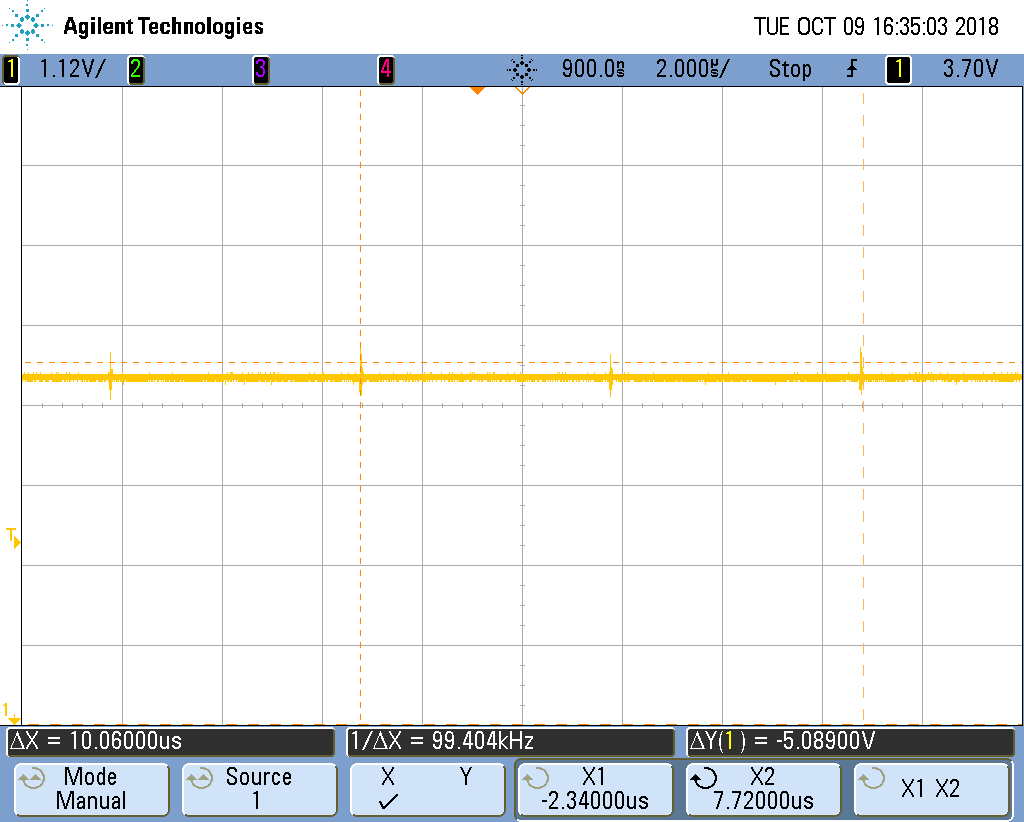
\includegraphics[scale=0.2]{imagenes/con_capacitor.png}
%\caption{Tensión en el terminal de alimentacion del 74HC02 con capacitor}
%\label{4_fig2} 
%\end{figure}

\begin{figure}[H]
\begin{center}
  \begin{minipage}[b]{0.4\textwidth}
  	\begin{center}
  		\includegraphics[scale=0.18]{imagenes/sin_capacitor.png}
  	\end{center}
  \caption{Tensión en el terminal de alimentacion del 74HC02 sin capacitor}
  \label{4_fig1} 
  \end{minipage}
  \begin{minipage}[b]{0.4\textwidth}
    \begin{center}
  		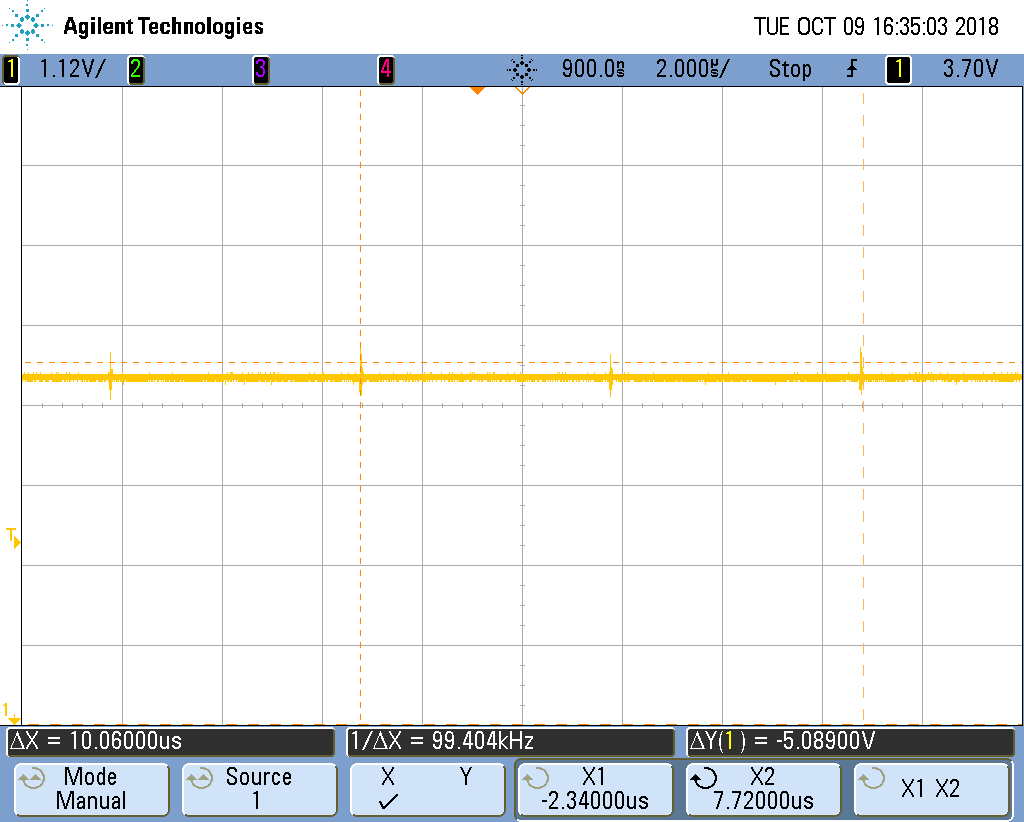
\includegraphics[scale=0.18]{imagenes/con_capacitor.png}
	\end{center}
  \caption{Tensión en el terminal de alimentacion del 74HC02 con capacitor}
  \label{4_fig2}
 \end{minipage}
\end{center}
\end{figure}






